\chapter{Modelling a Database for Dynamic Multimedia Data}
\label{chapter:system_model}


\section{Generalized Similarity Operations}

As has been argued in \Cref{chapter:theory_multimedia_analysis_and_retrieval}, there are two important assumptions for similiarity based operations, such as similarity search in multimedia retrieval. These assumptions can be summarized as follows:

\begin{itemize}
    \item For every object $o_{i}$ in a collection $\mathcal{C}$, there exists a feature transformation $\phi \colon \mathcal{C} \to \mathcal{F}$, that maps the object $o_{i} \in \mathcal{C}$ to a feature space $\mathcal{F}$.
    \item The feature space $\mathcal{F}$ and a to be defined distance function $\delta \colon \mathcal{F} \times \mathcal{F} \to \mathbb{R}$, constitute a metric space $(\mathcal{F},\delta)$, thus satisfying the identity of indiscernibles, symmetry and subadditivity condition.
\end{itemize}

For all similarity based operations, the output of $\delta$ -- i.e., the calculated distance $d$ -- acts as a proxy for (dis-)similiarty between two objects $o_{i}$, $o_{j} \in \mathcal{C}$ given the feature transformation $\phi$. Hence, the closer two objects $o_{i}$, $o_{j}$ appear under the transformation, the more (dis-)similar they are. It must be pointed out for the sake of completeness, that whether similarity is directly or inversely proportional to the distance is a matter of definition and depends on the concrete application. Also, in practice, multiple feature transformations $\phi_n$ may exist for a given media collection, leading to different feature spaces $\mathcal{F}_n$ for a collection $\mathcal{C}$ that must be considered jointly. Both these aspects are usually addressed by additional correspondence and scoring functions. Since both these aspects are not relevant for the discussion at hand, they will for now be ignored.

Using the relationship between (diss-)similarity and distance, it has been shown by Giangreco et al., that for a database to be able to support similarity-based search given the relational model for databases~\cite{Codd:1990Relational}, one can extend the data domain $\mathcal{D}$ by $\mathbb{R}^{dim}, dim \in \mathbb{N}$ and postulate the existence of a relational similarity operator $\tau_{\delta(\cdot,\cdot),a,q}(R)$ that \emph{``performs a similarity query under a distance $\delta(\cdot,\cdot)$ applied on an attribute $a$ of relation $R$ and compared to a query vector $q$.''} (\cite{Giangreco:2018thesis}, p. 138). Such an operation introduces an implicit attribute in the underlying relation $R$, which in turn induces an ascending ordering of the tuples. Using this operation, the authors then go on to define two concrete implementations, namely $\tau^{kNN}_{\delta(\cdot,\cdot),a,q}(R)$, and $\tau^{\epsilon NN}_{\delta(\cdot,\cdot),a,q}(R)$, which limit the number of retrieved results by their cardinality $k$ or a maximum cut-off distance $\epsilon$ respectively.

\subsection{Revisiting Distance Computation}

Considerding the definition provided in \Cref{chapter:theory_multimedia_analysis_and_retrieval}, we identify the following (implicit) constrained of the postulated model:

\begin{enumerate}
    \item The codomain (i.e., the output) of the distance function $\delta$ is assumed to be $\mathbb{R}$, hence, the distance value we generate is a real number.
    \item The domain (i.e., the input) of the distance function $\delta$ is assumed to be $\mathbb{R}^{dim} \times \mathbb{R}^{dim}$, hence, we restrict ourselves to real-valued vectors and the distance function is assumed to be a binary function.
\end{enumerate}

Upon further examination, one can see that there is very good reason to assume the codomain of $\delta$ to be in $\mathbb{R}$. On the one hand, it is obviously convenient both for the underlying mathematics as well as from a programming prespective. More importantly, however, real numbers -- unlike, for example, complex numbers or vectors -- come with a natural, total ordering, which is required for the sorting that is part of the relational similarity search operation. If, however, we turn to the use cases presented in \cref{section:application_retrieval} and \cref{section:application_mrf}, one can see that both the domain and the arity of a regular distance function are often too limited, as is shown in examples \cref{example:mrf} and \cref{example:svmdistance}.

\begin{example}[label=example:mrf]{Maximum Inner Product Search (MIPS) for MRF}{}
In MRF, we try to find the signal vector $f_i \in \mathcal{F}$ from a dictionary $\mathcal{F} \subset \mathbb{C}^{dim}$ so that it maximizes the inner product to a query vector $q \in \mathbb{C}^{dim}$. In this case, the distance function $\delta$ has the form $\delta \colon \mathbb{C}^{dim} \times \mathbb{C}^{dim} \to \mathbb{R}$ with $dim \in \mathbb{N}$.
\end{example}

\begin{example}[label=example:svmdistance]{Distance Between a Vector and a Hyperplane}{}
In the example introduced in \cref{section:application_retrieval}, want to find positive/negative examples for features in $\mathcal{F} \subset \mathbb{R}^{dim}$ given a linear classifier, e.g., provided by a SVM. Mathematically, such a classifier can be defined by a hyperplane $\mathbf{w}^T\mathbf{x} - b = 0$ with $\mathbf{w},\mathbf{x} \in \mathbb{R}^{dim}$ and $b \in \mathbb{R}$. The distance function can then be defined as $d \colon \mathbb{R}^{dim} \times \mathbb{R}^{dim} \times \mathbb{R} \to \mathbb{R}$ as both $\mathbf{w}$ and $b$ become parameters of the function, in addition to the attributes $f_i \in \mathcal{F}$ for which a distance is obtained. Hence, the distance function is no longer a binary but a ternay function with attributes $\mathbf{f_{i}}$, $\mathbf{w}$ and $b$.
\end{example}

In order to address these limitations, we propose the extension of a the distance function to the notion of a \emph{similarity proxy function (SPF)} following \cref{definition:spf}. As the name implies, such a function acts as a proxy for (dis-)similarity in similarity based operations.

\begin{definition}[label=definition:spf]{Similarity Proxy Function (SPF)}{}
    A \emph{similarity proxy function (SPF)} $\delta \colon \mathcal{F} \times \mathcal{F} \times \mathcal{D}_{1} ... \times \mathcal{D}_{n} \to \mathbb{R}$ is an n-ary but at least binary function that outputs a distance $d \in \mathbb{R}$ between an attribute $f_{a} \in \mathcal{F} \subset \mathcal{D}_i$ and a query $f_{q} \in \mathcal{D}_i$ using a well defined number of \emph{support arguments} from the data domains $\mathcal{D}_{j}$ with $i,j \in \mathbb{N}$.
\end{definition}

In simple terms, a SPF can be seen as a distance function that is being parametrized by its support arguments. A very simple and widely used example would be the Manhattan (L1) and the Euclidean (L2) distance, which are both parametrized versions of the more general Minkowski distance $\delta_{M} \colon \mathbb{R}^{dim} \times \mathbb{R}^{dim} \times \mathbb{N} \to \mathbb{R}$ with


\begin{equation}
    \delta_{L1}(\mathbf{q},\mathbf{f}) = \sum_{i=1}^{n} \mid q_i - f_i \mid = \left(\sum_{i=1}^{n} \mid q_i - f_i \mid^p\right)^{\frac{1}{p}}, p = 1
\end{equation}

\begin{equation}
    \delta_{L2}(\mathbf{q},\mathbf{f}) = \sqrt{\sum_{i=1}^{n} \mid q_i - f_i \mid^2}= \left(\sum_{i=1}^{n} \mid q_i - f_i \mid^p\right)^{\frac{1}{p}}, p = 2
\end{equation}


\begin{definition}[label=definition:spf]{Similarity Proxy Function (MSPF)}{}
    A SPF $\delta_{\mathcal{F}} \colon \mathcal{F} \times \mathcal{F} \times \mathcal{D}_{1} ... \times \mathcal{D}_{n} \to \mathbb{R}$ that fulfills the identity of indiscernibles, symmetry and subadditivity conditions with respect to $f_{a}  \in \mathcal{F} \subset \mathcal{D}_i$ and $f_{q} \in \mathcal{D}_i$ is called a \emph{metric similarity proxy function (MSPF)}. It induces a metric on the vector space $\mathcal{D}_j$.
\end{definition}

\subsubsection{Parametrized dimensionality}
As an aside, we must address the role of dimensionality in the case of vector spaces such as $\mathbb{R}^{dim}$ or $\mathbb{C}^{dim}$. One could argue, that the dimensionality of such a vector space can also be seens as a parameter of the SPF. Nevertheless, we consider the dimensionality to be a structural property of the underlying data domain as, for example, the data type. This means, that dimensionality as well as the type are well-defined and most importantly constant properties for a given relation.

\subsection{Extending the Relational Model}

Assuming the existence of an SPF as described in \cref{definition:spf}, one can start to integrate this into the relational algebra model. While postulating a new, relational operation $\tau^{kNN}_{\delta(\cdot,\cdot),a,q}(R)$ or $\tau^{\epsilon NN}_{\delta(\cdot,\cdot),a,q}(R)$ as proposed by \cite{Giangreco:2018thesis} has a certain elegance to it, it also comes with limitations that become apparent once we disect the structure of $\tau$. In its postulated form, $\tau$ addresses several functions at once:

\begin{enumerate}
    \item It specifies the distance function and its parameters.
    \item It generates an implicit distance attribute on the underlying relation $R$.
    \item It implies an implicit, ascending ordering on the tuples.
    \item It enforces a limit on the result set.
\end{enumerate}

While being very specific and thus straightforward to implement and optimize, the amalgamation of all this functionality into a single operation is very specifically tailored to the use-case of similarity search and only of limited value when considering more general similarity-based query operations. If we, for example, want to obtain the $k$ farthest neighbours rather than the $k$ nearest neighbours, as necessary when doing MIPS or obtaining negative examples, we would have to either change the distance function or extend the definition of $\tau$. Another important issue with the definition of $\tau$ in its current form is givn in Examples \ref{example:limitsoftauknn} and \ref{example:limitsoftauepsilonnn}.

\begin{example}[label=example:limitsoftauknn]{Shortcomings of $\tau^{kNN}_{\delta(\cdot,\cdot),a,q}$}{}
    Given a relation $R$ with $SCH(R) = \{ a_1, a_2 \}$, we consider the two relational expressions $\pi_{a1,d}(\tau^{kNN}_{\delta(\cdot,\cdot),a_2,q}(\sigma_{a_1 = true}(R)))$ and $\pi_{a1,d}(\sigma_{a_1 = true}(\tau^{kNN}_{\delta(\cdot,\cdot),a_2,q}(R)))$. 
    
    The keen observer will notice that for small numbers of $k$ with respect to the number of tuples that match the selection $\sigma$, the two expressions will not return the same resultset due to the order of execution. The first expression will always return a result set of size $k$ given that at least $k$ tuples in $R$ satisfy $\sigma$. The second expression, however, is likely to produce a resultset smaller than $k$ since the selection takes place on a top $k$ ranked subset of $R$.
\end{example}

\begin{example}[label=example:limitsoftauepsilonnn]{Shortcomings of $\tau^{\epsilon NN}_{\delta(\cdot,\cdot),a,q}$}{}
    Given a relation $R$ with $SCH(R) = \{ a_1, a_2 \}$, we consider the two relational expressions $\pi_{a1,d}(\tau^{\epsilon NN}_{\delta(\cdot,\cdot),a_2,q}(\sigma_{a_1 = true}(R)))$ and $\pi_{a1,d}(\sigma_{a_1 = true}(\tau^{\epsilon  NN}_{\delta(\cdot,\cdot),a_2,q}(R)))$, which select all entries that pass predicate $\sigma$ and whose distance $d \geq \epsilon$.
    
    Again, the keen observer will notice that the two result sets are going to be equal in this case. This can be attributed to the fact that the limiting of the resultset is formally introduced by another selection, i.e., the expression can be restated as $\pi_{a1,d}(\sigma_{d \geq \epsilon}(\tau_{\delta(\cdot,\cdot),a_2,q}(\sigma_{a_1 = true}(R))))$. It is perfectly valid to move the inner selection to the outside due to the commutativity of the selection operation. The only limitation is, that  $\sigma \geq \epsilon$ requires prior execution of $tau_{\delta(\cdot,\cdot),a_2,q}$.
\end{example}

With these example, we have demonstrated the limitations of $\tau$ and the fact that the two proposed implementations for $k$NN and $\epsilon$NN actually behave very differently despite their common core. We therefore propose to decompose $\tau$ into distinct extensions to the relational model, with a clear focus on separation of concerns.

\subsubsection{Extended Project and SPF}

First, we consider the SPF to be part of an \emph{extended projection} $\pi$, which has been defined as part of the extended relational algebra as described in \cref{section:relational_data_model}. In addition to projection on attributes, the extended projection allows for the projection on general algebraic expressions involving attributes, constants and function invocations. Given the extended projection, the invocation of a SPF can be expressed as follows.

\begin{definition}[label=definition:spf_rel]{Similarity Proxy Function (SPF) in Extended Projection}{}
Let $\delta \colon \mathcal{F} \times \mathcal{F} \times \mathcal{D}_{1} ... \times \mathcal{D}_{n-2} \to \mathbb{R}$ be an SPF and $R$ be a relation with $SCH(R) = \{ a_1, a_2, ... a_{n} \}$. The \emph{extended projection} $\pi_{\delta(a_1,a_2,...,a_n)}$(R) describes
the execution of the n-ary SPF $\delta$ using attributes $a_1,a_2,...a_n$ from relation $R$ as parameters. Note that $\pi_{\delta(a_1,a_2,...,a_n)}$ introduces a new, calculated distance attribute $a_d \in \mathbb{R}$ on each tuple $t_i \in R$, i.e., $SCH(\pi_{\delta(a_1,a_2,...,a_n), a_1, a_2, ..., a_n}) = SCH(R) \cup \{ a_d \}$.
\end{definition}




Obviously, the combination of multiple SPF in a single, extended projection or the combination of simple attribute projection with SPFs are also allowed. Hence, the following expressions are valid examples of the extended projection on relation $R$ with $SCH(R) = \{ a_1, a_2, a_3, a_4 \}$: $\pi_{\delta_1(a_1,a_2), \delta_2(a_2,a_3,a_1)}(R)$ or $\pi_{\delta(a_1,a_2), a_3, a_4}(R)$ or $\pi_{a_1, a_3, a_4}(R)$.


\begin{itemize}
    \item NNS: Scan -> (Predicate) -> Distance Function -> Sort -> Limit -> (Predicate); no need for dedicated language feature aside from distance function
    \item Distance function is a binary function $D(q,v) \longrightarrow d$, $q$ and $v$ can be elements of $\mathbb{R}^d,\mathbb{C}^d$ or some other object (e.g. matrices)
    \item Different types of distance functions, depending on parameters they accept; e.g. distance between point \& point or point \& plane etc.
    \item Systems perspective 1: How enable planner to reason about distance function execution? Possible optimizations?
    \item Systems perspective 2: Concrete applications in multimedia retrieval and analytics?
\end{itemize}

\section{Cost Model for Retrieval Accuracy}
Describe cost model for execution plans with following properties:

\begin{itemize}
    \item Cost as a function of atomic costs: $f(a_{cpu}, a_{io}, a_{memory}, a_{accuracy}) \longrightarrow C$
    \item Means to estimate results accuracy and associated considerations from execution path (e.g., when using index) based on properties of the index
    \item Means to specify importance of accurate results (e.g., global, per-query, context-based i.e. when doing 1NN search) in comparison to other factors
    \item Systems perspective 1: How can such a cost model be applied during query planning and optimization?
\end{itemize}

\section{Adaptive Index Management}

\begin{figure}[h!]
    \centering
    \begin{subfigure}[b]{0.40\textwidth}
        \centering
        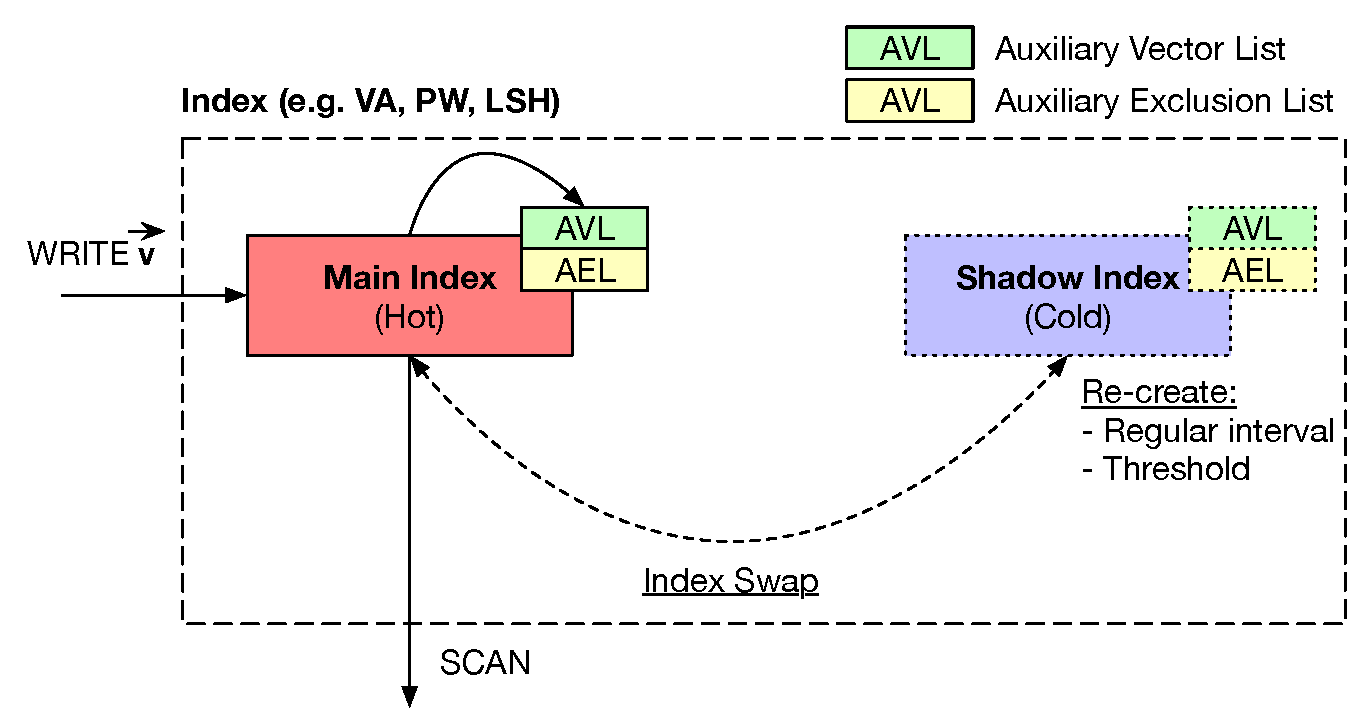
\includegraphics[width=\textwidth]{figures/adaptive_index.eps}
        \label{fig:adaptive_index:architecture}
    \end{subfigure}
    \hfill
    \begin{subfigure}[b]{0.40\textwidth}
        \centering
        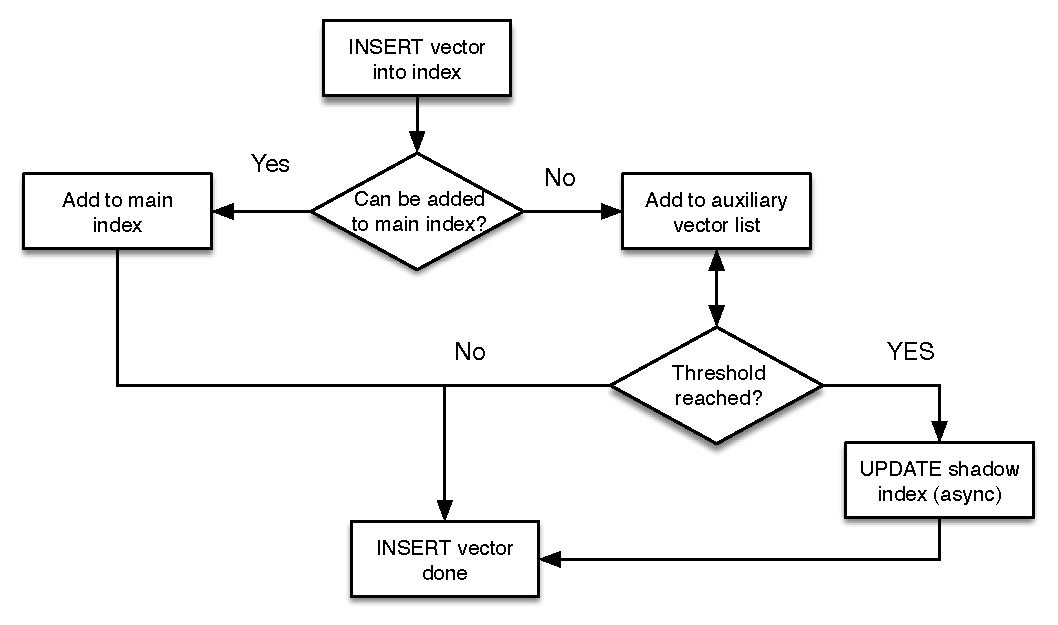
\includegraphics[width=\textwidth]{figures/adaptive_index_flow.eps}
        \label{fig:adaptive_index:flow}
    \end{subfigure}
    \caption{Adaptive index structures overview.}
    \label{fig:adaptive_index}
\end{figure}

Describe model for index management in the face of changing data (adaptive index management):

\begin{itemize}
    \item Reason about properties of secondary indexes for NNS (e.q., PQ, VA, LSH) with regards to data change
    \item Derivation of error bounds possible (e.g., usable for planning)?! Use in query planning?
    \item Systems perspective 1: How to cope with ``dirty'' indexes? Proposal: hot vs. cold index, auxilary data structure, offline optimization, see \cref{fig:adaptive_index}
    \item Systems perspective 2: On-demand index based on query workload?
\end{itemize}

\section{Architecture Model}

\todo[inline]{Putting everything together into a unified systems model (base on previous work + aforementioned aspects).}




